% Provenance (never printed): see sources/outline_sources.md and sources/book1/BRIEFS.md (g2/01).
\chapter{The Keyboard and the Mouse}\label{ch:g2:keyboard-and-mouse}

Lina sits at the family \omterm{def:g1:what-is-a-computer:computer}{computer} to type her name for the first time. She
finds the L and presses it: a small ``l'' appears on the screen, not the
capital she wanted. Then she wants to write her surname on the next line, so
she presses the long \omterm{def:g2:keyboard-and-mouse:key}{key} at the bottom of the keyboard. A space appears, and
the surname stays on the same line. The keyboard has more than a hundred \omterm{def:g2:keyboard-and-mouse:key}{keys}:
which one does what?

\begin{recall}
The keyboard, the mouse and the \omterm{def:g2:keyboard-and-mouse:touchpad}{touchpad} are \omterm{def:g1:what-is-a-computer:device}{input devices}: they bring
information into the \omterm{def:g1:what-is-a-computer:computer}{computer}. A \omterm{def:g2:keyboard-and-mouse:touchpad}{touch screen} is both an \omterm{def:g1:what-is-a-computer:device}{input device} and an
\omterm{def:g1:what-is-a-computer:device}{output device} (\cref{ch:g1:what-is-a-computer}).
\end{recall}

\section{The keys}

\begin{definition}[Key of a keyboard]\label{def:g2:keyboard-and-mouse:key}
A \emph{key}\index{key (keyboard)} is one button of a keyboard. Pressing a
key sends one \omterm{def:g1:what-is-a-computer:input}{input} to the \omterm{def:g1:what-is-a-computer:computer}{computer}: a letter, a digit, a sign, or an order
such as ``start a new line''.
\end{definition}

When you type, the letters appear at one place in the text: the place of the
\omterm{def:g2:keyboard-and-mouse:cursor}{cursor}.

\begin{definition}[Cursor]\label{def:g2:keyboard-and-mouse:cursor}
The \emph{cursor}\index{cursor} is the small blinking line in a text that
shows where the next letter you type will appear.
\end{definition}

The \omterm{def:g2:keyboard-and-mouse:key}{keys} of a keyboard come in groups. Most of them type something; a few of
them change what the other \omterm{def:g2:keyboard-and-mouse:key}{keys} do or move the \omterm{def:g2:keyboard-and-mouse:cursor}{cursor}.
\begin{itemize}
\item The \textbf{letter \omterm{def:g2:keyboard-and-mouse:key}{keys}} type small letters: a, b, c\dots
\item The \textbf{digit \omterm{def:g2:keyboard-and-mouse:key}{keys}}, in the top row, type 0, 1, 2\dots\ 9.
\item The \textbf{space bar}, the long \omterm{def:g2:keyboard-and-mouse:key}{key} at the bottom, types a space
between two words.
\item \key{Enter} starts a new line.
\item \key{Backspace} rubs out the letter just before the \omterm{def:g2:keyboard-and-mouse:cursor}{cursor};
\key{Delete} (on many keyboards) rubs out the letter just after it.
\item \key{Shift} is held down while another \omterm{def:g2:keyboard-and-mouse:key}{key} is pressed: then a letter
\omterm{def:g2:keyboard-and-mouse:key}{key} types a capital, and a digit \omterm{def:g2:keyboard-and-mouse:key}{key} types the sign drawn above the digit.
\item \key{Caps Lock}, pressed once, makes every letter a capital until it is
pressed again.
\item The four \textbf{arrow \omterm{def:g2:keyboard-and-mouse:key}{keys}}, usually at the bottom right, move the
\omterm{def:g2:keyboard-and-mouse:cursor}{cursor} up, down, left and right, without typing anything.
\end{itemize}

\begin{omfigure}
\begin{tikzpicture}[font=\small, lab/.style={draw=black!60, fill=white, rounded corners=2pt, inner sep=2pt, font=\footnotesize}]
  \omkeyboardkeys[unit=0.78cm, highlight={LFSH,RTSH,RTRN,BKSP,SPCE,CAPS}]{us}
  \node[lab] (dig) at (2.4,1.1) {digit keys};
  \draw[black!60] (dig) -- (kb-AE03.north);
  \node[lab] (let) at (7.0,1.1) {letter keys};
  \draw[black!60] (let) -- (kb-AD06.north);
  \node[lab] (bk) at (10.6,1.1) {Backspace};
  \draw[black!60] (bk) -- (kb-BKSP.north);
  \node[lab] (en) at (12.9,-0.15) {Enter};
  \draw[black!60] (en) -- (kb-RTRN.north);
  \node[lab] (sh) at (-1.3,-2.9) {Shift};
  \draw[black!60] (sh) -- (kb-LFSH.west);
  \node[lab] (cl) at (-1.5,-1.9) {Caps Lock};
  \draw[black!60] (cl) -- (kb-CAPS.west);
  \node[lab] (sp) at (5.2,-4.7) {space bar};
  \draw[black!60] (sp) -- (kb-SPCE.south);
\end{tikzpicture}

{\small The main \omterm{def:g2:keyboard-and-mouse:key}{keys} of a keyboard. The \omterm{def:g2:keyboard-and-mouse:key}{keys} that change what other \omterm{def:g2:keyboard-and-mouse:key}{keys} do,
or that do not type a letter, are outlined. On your keyboard the letters may be
in another order: this drawing shows one common keyboard.}
\label{fig:g2:keyboard-and-mouse:keyboard}
\end{omfigure}

\begin{example}[Typing ``Lina'' with a capital]\label{ex:g2:keyboard-and-mouse:capital}
Hold \key{Shift} down with one hand, press L with the other, then let go of
\key{Shift}: a capital L appears. Then press i, n, a. If you made a mistake,
press \key{Backspace} once to rub out the last letter, and type it again. To
write the surname on the next line, press \key{Enter}, not the space bar.
\end{example}

\section{Sitting well}

We may spend a long time in front of a \omterm{def:g1:what-is-a-computer:computer}{computer}, so it is worth sitting well.

\begin{method}[A good position at the computer]\label{met:g2:keyboard-and-mouse:posture}
% ledger: g2:screen-distance, g2:screen-height
Sit with your back against the back of the chair and your feet flat on the
floor (or on a footrest). Keep your forearms level, with your hands resting
loosely on the keyboard. Put the screen straight in front of you, at least an
arm's length away, with its top at the height of your eyes or a little lower.
Every so often, look far away and stand up for a moment.
\end{method}

\begin{omfigure}
\begin{tikzpicture}[x=1cm, y=1cm, font=\footnotesize, lab/.style={align=left, font=\footnotesize}]
  % floor, desk, chair
  \draw[black!50, thick] (-1,0) -- (8,0);
  \draw[black!60, fill=black!8] (3.2,2.6) rectangle (7.2,2.75);
  \draw[black!60] (3.4,2.6) -- (3.4,0); \draw[black!60] (7.0,2.6) -- (7.0,0);
  \draw[black!60, fill=black!8] (0.2,1.5) rectangle (2.0,1.65);
  \draw[black!60, line width=1.2pt] (0.25,1.5) -- (0.25,3.3);
  \draw[black!60] (1.1,1.5) -- (1.1,0.2) -- (0.5,0) (1.1,0.2) -- (1.7,0);
  % screen
  \draw[black!70, fill=ocPaleBlue] (6.1,2.95) rectangle (6.25,3.85);
  \draw[black!60] (6.17,2.75) -- (6.17,2.95);
  % keyboard
  \draw[black!60, fill=black!20] (3.6,2.75) rectangle (4.4,2.85);
  % child (stick figure)
  \draw[ocBlue!70!black, line width=2pt, line cap=round]
    (0.55,1.75) -- (0.6,3.4)      % back
    (0.55,1.75) -- (1.95,1.8)     % thigh
    (1.95,1.8) -- (2.05,0.35)     % shin
    (2.05,0.35) -- (2.45,0.3)     % foot
    (0.62,3.25) -- (0.95,2.88)    % upper arm
    (0.95,2.88) -- (3.8,2.88);    % forearm, level
  \fill[ocBlue!70!black] (0.68,3.75) circle (0.32);
  \fill[white] (0.88,3.82) circle (0.05);
  % eye line and distance
  \draw[ocRed!80!black, dashed] (0.95,3.82) -- (6.6,3.82);
  \draw[ocRed!80!black, {Stealth[length=2mm]}-{Stealth[length=2mm]}] (0.95,4.75) -- (6.1,4.75);
  \node[text=ocRed!80!black, fill=white, inner sep=1pt] at (3.5,4.75) {at least an arm's length};
  \node[lab, anchor=west] at (6.6,3.82) {top of the screen\\near eye height};
  \node[lab, anchor=east] at (-0.1,2.7) {back against\\the chair};
  \node[lab, anchor=south] at (2.4,2.95) {forearms level};
  \node[lab, anchor=north] at (2.3,-0.05) {feet flat};
\end{tikzpicture}

{\small Sitting well at a \omterm{def:g1:what-is-a-computer:computer}{computer}, seen from the side.}
\label{fig:g2:keyboard-and-mouse:posture}
\end{omfigure}

\begin{omfigure}
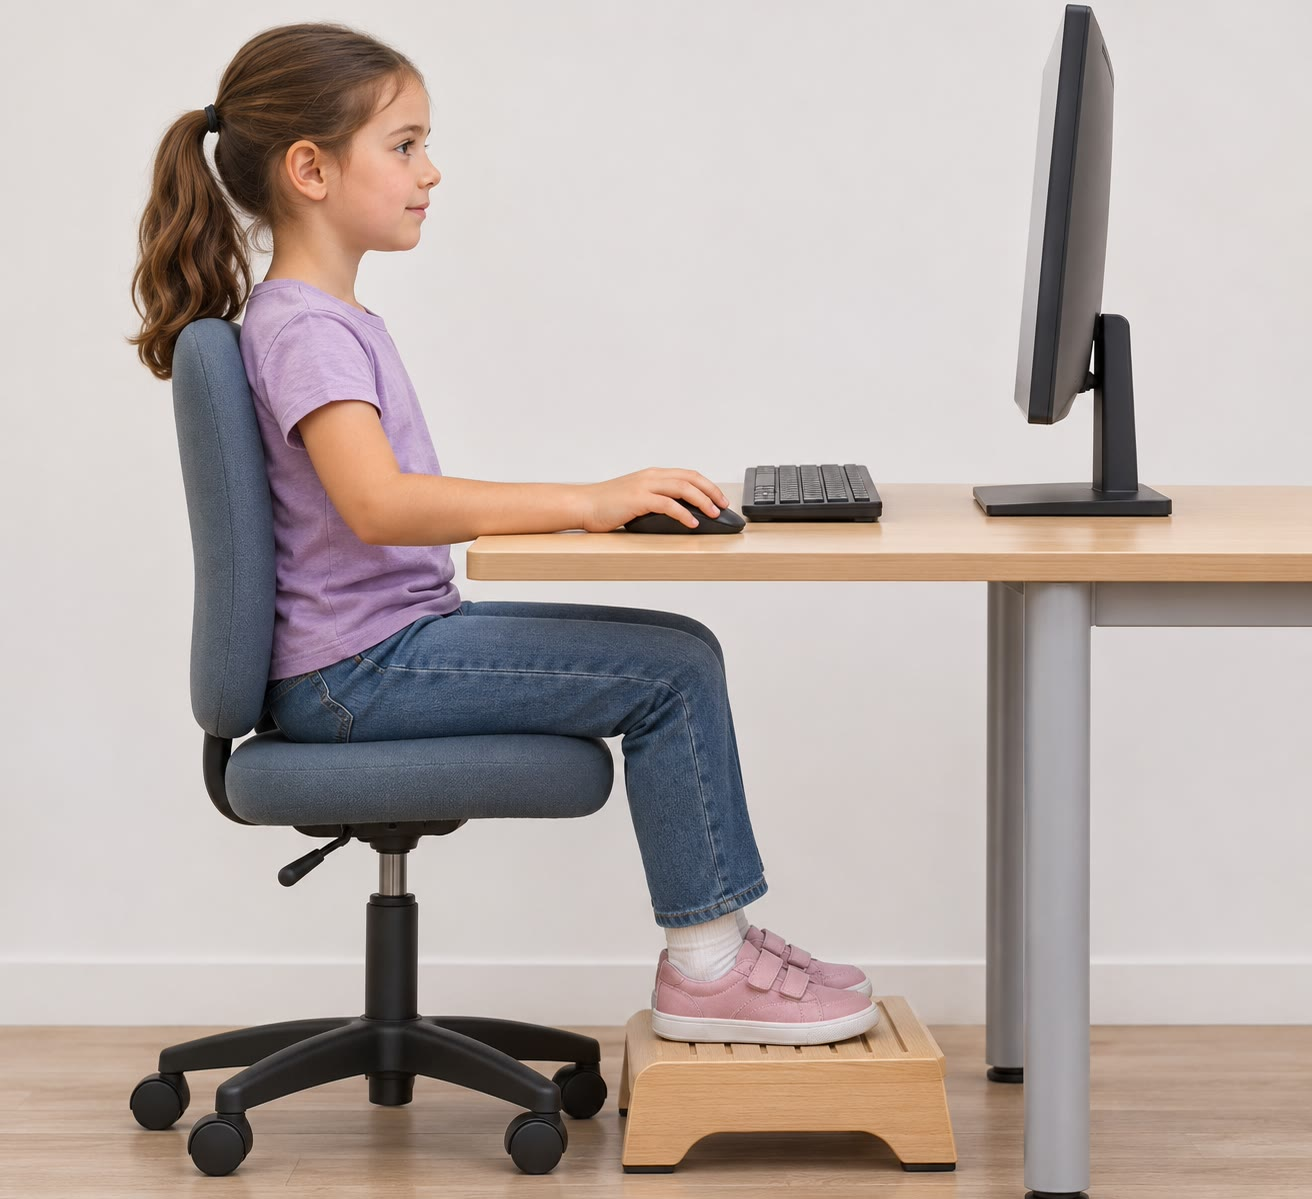
\includegraphics[width=0.58\linewidth]{images/book1/ai/g2-keyboard-and-mouse-sitting-well.jpg}

{\small A child sitting well: back against the chair, feet on a footrest,
forearms level, the screen in front at an arm's length.}
\end{omfigure}

\section{The pointer}

When you move the mouse on the table, a small arrow moves the same way on the
screen.

\begin{definition}[Pointer]\label{def:g2:keyboard-and-mouse:pointer}
The \emph{pointer}\index{pointer} is the small arrow on the screen that moves
when you move the mouse or your finger on the \omterm{def:g2:keyboard-and-mouse:touchpad}{touchpad}. It shows what the
next \omterm{def:g2:keyboard-and-mouse:click}{click} will act on.
\end{definition}

Do not mix up the \omterm{def:g2:keyboard-and-mouse:cursor}{cursor} and the \omterm{def:g2:keyboard-and-mouse:pointer}{pointer}. The \omterm{def:g2:keyboard-and-mouse:cursor}{cursor} is in a text and shows
where the next letter goes; it moves when you type or use the arrow \omterm{def:g2:keyboard-and-mouse:key}{keys}. The
\omterm{def:g2:keyboard-and-mouse:pointer}{pointer} can go anywhere on the screen; it moves with the mouse.

\begin{definition}[Click, double-click, drag]\label{def:g2:keyboard-and-mouse:click}
To \emph{click}\index{click} is to press the main button of the mouse and let
it go at once, without moving. To \emph{double-click}\index{double-click} is
to click twice, quickly, at the same place. To \emph{drag}\index{drag} is to
press the button, keep it pressed while moving the mouse, and let it go at
the new place.
\end{definition}

A \omterm{def:g2:keyboard-and-mouse:click}{click} usually chooses something: a button, a word, a place in a text. A
\omterm{def:g2:keyboard-and-mouse:click}{double-click} often opens something. Dragging moves something, for example a
picture, from one place to another. Most mice have a second button, on the
right: a \omterm{def:g2:keyboard-and-mouse:click}{right-click} opens a short list of choices.

\begin{omfigure}
\begin{tikzpicture}[x=1cm, y=1cm, font=\footnotesize,
    dn/.style={draw=black!60, fill=ocBlue!45, rounded corners=2pt, minimum width=1.25cm, minimum height=6mm},
    up/.style={draw=black!60, fill=white, rounded corners=2pt, minimum width=1.25cm, minimum height=6mm},
    mv/.style={draw=black!60, fill=ocYellow!50, rounded corners=2pt, minimum width=1.25cm, minimum height=6mm}]
  \node[anchor=east, font=\small\bfseries] at (-0.3,2) {click};
  \node[dn] at (0.7,2) {press}; \node[up] at (2.1,2) {release};
  \node[anchor=east, font=\small\bfseries] at (-0.3,1) {double-click};
  \node[dn] at (0.7,1) {press}; \node[up] at (2.1,1) {release};
  \node[dn] at (3.5,1) {press}; \node[up] at (4.9,1) {release};
  \node[anchor=west] at (5.7,1) {quickly, same place};
  \node[anchor=east, font=\small\bfseries] at (-0.3,0) {drag};
  \node[dn] at (0.7,0) {press};
  \node[mv, minimum width=2.6cm] at (2.75,0) {move, still pressed};
  \node[up] at (4.8,0) {release};
  \draw[-{Stealth[length=2mm]}, black!50] (0,-0.6) -- (6.6,-0.6) node[right] {time};
\end{tikzpicture}

{\small Three things to do with the mouse button, from left to right in time.
Blue: the button is held down; white: it is let go.}
\label{fig:g2:keyboard-and-mouse:actions}
\end{omfigure}

\section{Touchpad and touch screen}

\begin{definition}[Touchpad and touch screen]\label{def:g2:keyboard-and-mouse:touchpad}
A \emph{touchpad}\index{touchpad} is a flat square below the \omterm{def:g2:keyboard-and-mouse:key}{keys} of a laptop:
moving one finger on it moves the \omterm{def:g2:keyboard-and-mouse:pointer}{pointer}, and a tap on it is a \omterm{def:g2:keyboard-and-mouse:click}{click}. A
\emph{touch screen}\index{touch screen} is a screen that feels where it is
touched: the finger itself is the \omterm{def:g2:keyboard-and-mouse:pointer}{pointer}.
\end{definition}

\begin{omfigure}
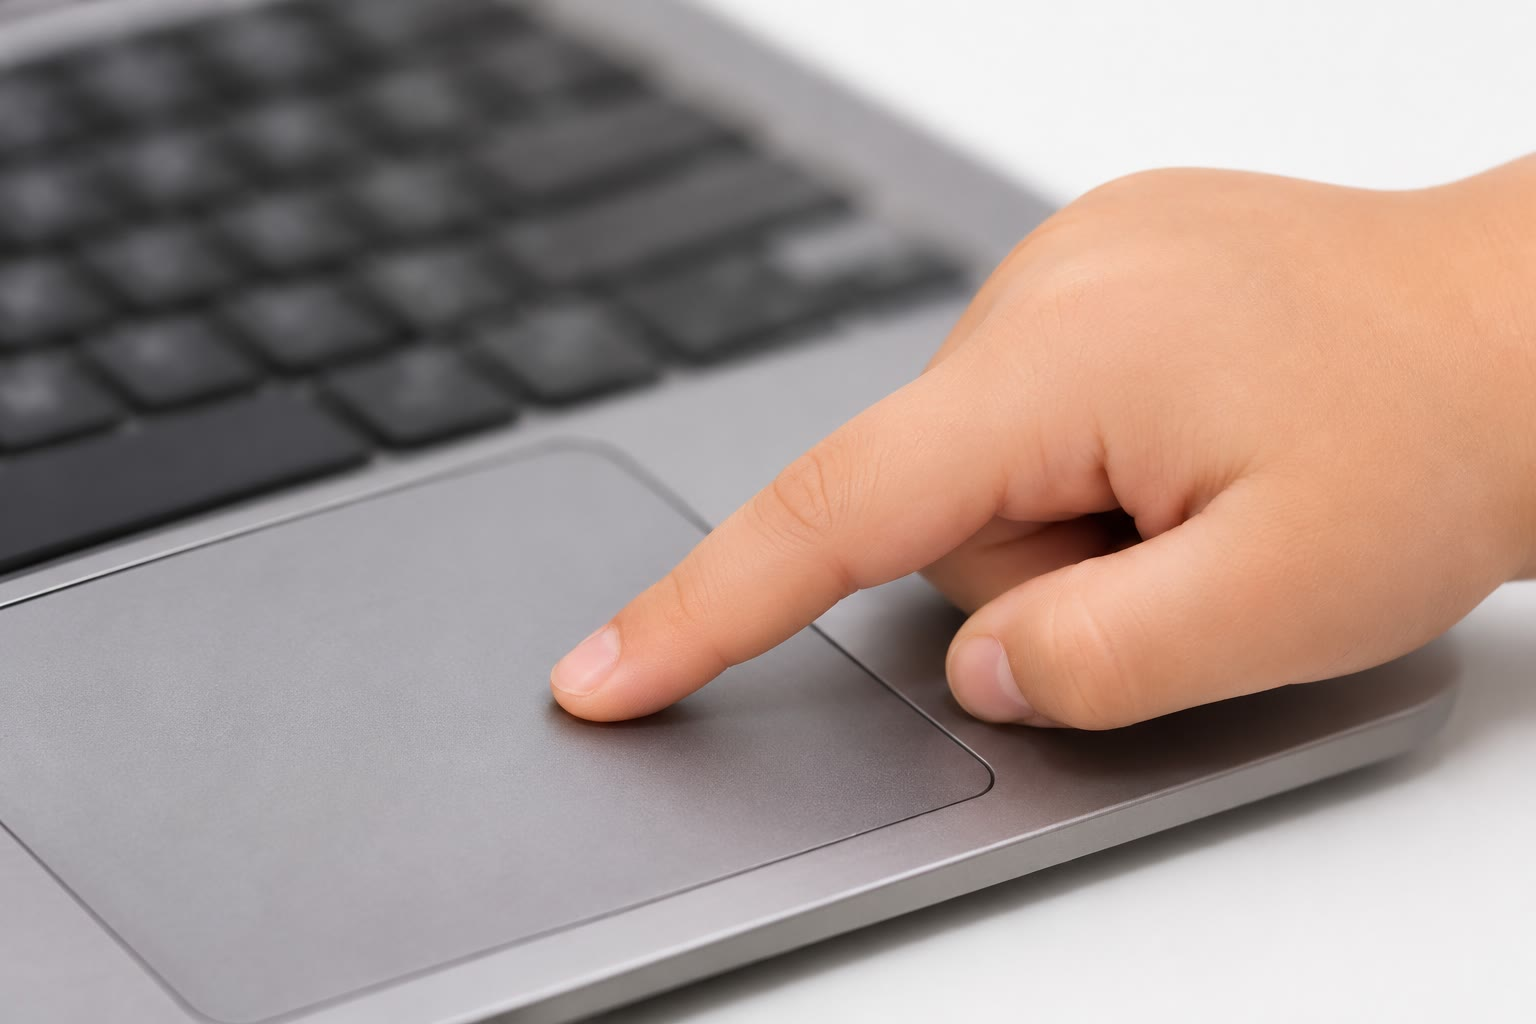
\includegraphics[width=0.55\linewidth]{images/book1/ai/g2-keyboard-and-mouse-touchpad.jpg}

{\small One finger on the \omterm{def:g2:keyboard-and-mouse:touchpad}{touchpad} of a laptop moves the \omterm{def:g2:keyboard-and-mouse:pointer}{pointer} on the
screen.}
\end{omfigure}

On a \omterm{def:g2:keyboard-and-mouse:touchpad}{touch screen}, there is no \omterm{def:g2:keyboard-and-mouse:pointer}{pointer} to move: you touch the thing you want.
\begin{itemize}
\item A \textbf{tap} (touch and lift at once) is like a \omterm{def:g2:keyboard-and-mouse:click}{click}.
\item \textbf{Press and hold} (keep the finger still for a second) is like a
\omterm{def:g2:keyboard-and-mouse:click}{right-click}: it often shows a list of choices.
\item A \textbf{swipe} (slide one finger) moves the page or turns to the next
picture.
\item A \textbf{pinch} (move two fingers apart or together) makes a picture
bigger or smaller.
\end{itemize}

\section{Exercises}

\begin{exercise}[$\star$]\label{exo:g2:keyboard-and-mouse:1}
Which \omterm{def:g2:keyboard-and-mouse:key}{key} do you use: (a)~to type a capital? (b)~to rub out the letter just
before the \omterm{def:g2:keyboard-and-mouse:cursor}{cursor}? (c)~to start a new line?
\end{exercise}

\begin{exercise}[$\star$]\label{exo:g2:keyboard-and-mouse:2}
Look at your own keyboard. What do you think \key{Shift} + 1 types on it? Look
at the \omterm{def:g2:keyboard-and-mouse:key}{key}: what is drawn on it, above the 1?
\end{exercise}

\begin{exercise}[$\star$]\label{exo:g2:keyboard-and-mouse:3}
What is the difference between the \omterm{def:g2:keyboard-and-mouse:cursor}{cursor} and the \omterm{def:g2:keyboard-and-mouse:pointer}{pointer}?
\end{exercise}

\begin{exercise}[$\star$]\label{exo:g2:keyboard-and-mouse:4}
Name each action: (a)~press, release; (b)~press, move with the button still
pressed, release; (c)~press, release, press, release, quickly.
\end{exercise}

\begin{exercise}[$\star$]\label{exo:g2:keyboard-and-mouse:5}
Tom sits at the \omterm{def:g1:what-is-a-computer:computer}{computer} with his back bent forward, his feet hanging under the
chair, and his nose close to the screen. Name three things he should change.
\end{exercise}

\begin{exercise}[$\star$]\label{exo:g2:keyboard-and-mouse:6}
On a tablet, which movement do you use: (a)~to open a game? (b)~to see the
next photo? (c)~to make a photo bigger?
\end{exercise}

\begin{exercise}[$\star$]\label{exo:g2:keyboard-and-mouse:7}
In the drawing of the keyboard, where are \key{Backspace}, \key{Enter} and the
space bar? Which of these \omterm{def:g2:keyboard-and-mouse:key}{keys} does not type anything?
\end{exercise}

\begin{exercise}[$\star$]\label{exo:g2:keyboard-and-mouse:8}
What does a \omterm{def:g2:keyboard-and-mouse:touchpad}{touchpad} replace on a laptop? How do you \omterm{def:g2:keyboard-and-mouse:click}{click} with it?
\end{exercise}

\begin{exercise}[$\star\star$]\label{exo:g2:keyboard-and-mouse:9}
List, in order, every \omterm{def:g2:keyboard-and-mouse:key}{key} you press to type \code{Hi Sam}.
\end{exercise}

\begin{exercise}[$\star\star$]\label{exo:g2:keyboard-and-mouse:10}
Mia wants to move a picture to the other side of her drawing. Should she \omterm{def:g2:keyboard-and-mouse:click}{click}
on it or \omterm{def:g2:keyboard-and-mouse:click}{drag} it? What happens if she only \omterm{def:g2:keyboard-and-mouse:click}{clicks}?
\end{exercise}

\begin{exercise}[$\star\star$]\label{exo:g2:keyboard-and-mouse:11}
Leo typed ``mY NAME IS lEO''. What happened? How can he type the sentence
correctly?
\end{exercise}
